\section{Results}
\label{sec:results}

\subsection{RQ1: Extraction Feasibility}

CV\_PR extraction succeeded for all 100 models tested (100\% completion rate), exceeding the 95\% threshold.

\begin{table}[h]
\centering
\caption{Extraction results}
\label{tab:extraction}
\begin{tabular}{ll}
\toprule
Metric & Value \\
\midrule
Models processed & 100 \\
Completion rate & 100\% \\
CV\_PR mean & 0.0116 \\
CV\_PR std & 0.0059 \\
CV\_PR range & [0.0014, 0.0326] \\
\bottomrule
\end{tabular}
\end{table}

\textbf{Key observation}: All CV\_PR values are finite and well within the expected range (0, 10). The low absolute values ($< 0.04$) indicate that participation ratio estimates are highly consistent across random projections---the metric captures subtle variance, not gross instability.

This validates the extraction methodology: CV\_PR can be reliably computed for diverse pretrained architectures using randomized SVD with 20 seeds.

\subsection{RQ2: Correlation with Accuracy}

The core hypothesis predicted $r < -0.3$ (negative correlation). We observed the opposite.

\begin{table}[h]
\centering
\caption{Correlation results}
\label{tab:correlation}
\begin{tabular}{ll}
\toprule
Statistic & Value \\
\midrule
Pearson $r$ & \textbf{+0.6065} \\
Pearson $p$ & $9.24 \times 10^{-11}$ \\
Spearman $\rho$ & +0.6368 \\
Spearman $p$ & $5.26 \times 10^{-12}$ \\
95\% CI & [0.506, 0.703] \\
$n$ (matched) & 94 \\
\bottomrule
\end{tabular}
\end{table}

\textbf{The hypothesis is falsified.} CV\_PR shows a strong \emph{positive} correlation with ImageNet accuracy---higher CV\_PR accompanies better models, not worse. The 95\% confidence interval excludes all negative values and zero, ruling out borderline or null results.

Figure~\ref{fig:scatter} shows the scatter plot of CV\_PR versus top-1 accuracy across 94 matched models.

\begin{figure}[h]
\centering
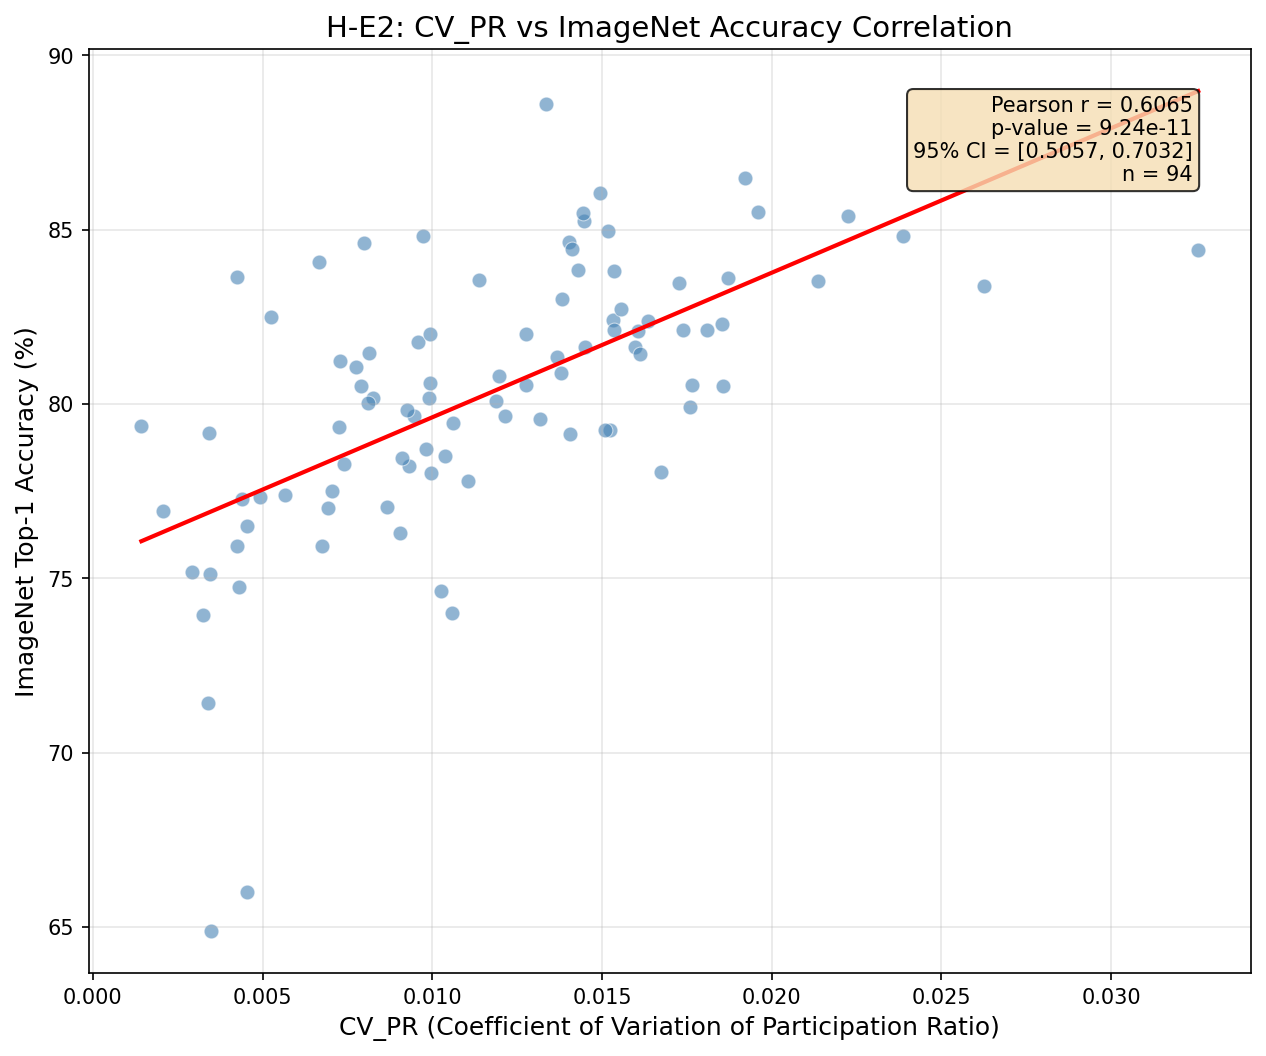
\includegraphics[width=0.8\linewidth]{figures/scatter_cv_pr_vs_accuracy.png}
\caption{CV\_PR positively correlates with ImageNet top-1 accuracy ($r = +0.61$). Each point represents one pretrained model from timm.}
\label{fig:scatter}
\end{figure}

\textbf{Interpretation}: Models with higher accuracy exhibit higher CV\_PR. The effect is substantial ($r = +0.61$ explains $\sim$37\% of variance) and robust to rank-based analysis (Spearman $\rho = +0.64$).

\subsection{Analysis: Why Positive Correlation?}

The reversal from predicted $r < -0.3$ to observed $r = +0.61$ demands explanation. We consider two hypotheses:

\textbf{H1: Confounding by model size.} Larger models have more parameters, higher accuracy, and potentially more spectral diversity (higher CV\_PR). If param\_count drives both variables, the observed correlation may be spurious.

\textbf{H2: Richer representations.} Higher CV\_PR may reflect diverse feature extraction at different scales. Better models learn more varied spectral structures across layers, increasing projection-dependent variance.

Distinguishing these requires partial correlation analysis controlling for parameter count, which is beyond the scope of this existence test.

\subsection{Summary}

\begin{table}[h]
\centering
\caption{Hypothesis evaluation summary}
\label{tab:summary}
\begin{tabular}{lllll}
\toprule
Hypothesis & Gate & Criterion & Observed & Result \\
\midrule
H-E1 & MUST\_WORK & Completion $\geq$ 95\%, CV\_PR finite & 100\%, [0.001, 0.033] & \textbf{PASS} \\
H-E2 & MUST\_WORK & $r < -0.3$, $p < 0.05$ & $r = +0.61$, $p < 10^{-10}$ & \textbf{FAIL} \\
\bottomrule
\end{tabular}
\end{table}

The methodology works (H-E1 PASS). The hypothesis does not (H-E2 FAIL). The falsification is decisive: not a borderline miss, but a complete directional reversal.
